% easychair.tex,v 3.5 2017/03/15

\documentclass[a4paper]{easychair}

\usepackage{doc}

% use this if you have a long article and want to create an index
% \usepackage{makeidx}

% In order to save space or manage large tables or figures in a
% landcape-like text, you can use the rotating and pdflscape
% packages. Uncomment the desired from the below.
%
% \usepackage{rotating}
% \usepackage{pdflscape}

%\makeindex

%% Front Matter
%%
% Regular title as in the article class.
%
\title{Heterogeneous behavioral model composition \\
        using graph grammars}

% Authors are joined by \and. Their affiliations are given by \inst, which indexes
% into the list defined using \institute
%
\author{
Tim Kräuter
}

% Institutes for affiliations are also joined by \and,
\institute{
  Høgskulen på Vestlandet\\
  Bergen, Norway\\
  \email{tkra@hvl.no}
 }

%  \authorrunning{} has to be set for the shorter version of the authors' names;
% otherwise a warning will be rendered in the running heads. When processed by
% EasyChair, this command is mandatory: a document without \authorrunning
% will be rejected by EasyChair

\authorrunning{Tim Kräuter}

% \titlerunning{} has to be set to either the main title or its shorter
% version for the running heads. When processed by
% EasyChair, this command is mandatory: a document without \titlerunning
% will be rejected by EasyChair
\titlerunning{Heterogeneous behavioral model composition}

\usepackage{glossaries}

\newacronym{mde}{MDE}{Model-driven engineering}
\newacronym[
    shortplural={GG's},
    longplural={graph grammars}
]{gg}{GG}{graph grammar}
\newacronym{bpmn}{BPMN}{Business Process Modeling Notation}
\newacronym{ct}{CT}{category theory}
\newacronym{uml}{UML}{Unified Modeling Language}
\newacronym{dsl}{DSL}{Domain Specific Language}
\newacronym{csp}{CSP}{Communication Sequential Processes}

\begin{document}

\maketitle
% 2-3 pages abstract wanted by NWPT

%------------------------------------------------------------------------------
\section{Introduction}
% Introduction/Motivation
A common approach to handle the increasing complexity of software systems is \gls{mde}.
\gls{mde} leads to a clear separation of concerns by modeling each aspect of a system separately \cite{franceModeldrivenDevelopmentComplex2007}.
However, these individual models must be composed if one wants to execute the system or argue about global properties \cite{kienzleUnifyingFrameworkHomogeneous2019}.

% Narrowing down
Our contribution addresses the problem of how the individual models can be composed into one model describing the entire software system, even if the used models are heterogeneous, i.e., do not conform to the same modeling language.
In particular, we address the composition of behavioral models since its structural counterpart has been the focus of a significant amount of research already, for example, in \cite{kienzleUnifyingFrameworkHomogeneous2019, klareCommonalitiesPreservingConsistency2019, stunkelComprehensiveSystemsFormal2021}.
We further limit the behavioral models to those describing discrete behavior such as finite state machines, \gls{bpmn} diagrams, process algebras, and Petri nets. % Untimed variants and only a subset of BPMN.

\section{Heterogeneous behavioral model composition}
We assume that each behavioral model describes a component of the overall system running independently and in parallel to other components as long as no relation to any other component is defined.
However, components, i.e., behavioral models, must interact to realize a meaningful composite system behavior.

% We suggest 2 primitives to relate behavioral models: synchronous and asynchronous communication (currently without data).
Our approach supports two types of interactions between behavioral models: \textit{synchronous} and \textit{asynchronous} communication.
One can use synchronous communication to model that one component acquires a resource realized as a separate model since it is shared across the entire system.
Asynchronous communication can, for example, be used to model that two components communicate using a messaging system or by writing/consuming files in a shared file system.
Defining synchronous communication leads to two components becoming active simultaneously, while asynchronous communication only requires one component to be active. 

Our model composition approach can be separated into three steps.
% 1. Step: Relate models by defining interactions.
The first step is to define interactions among a set of behavioral models using synchronous and asynchronous communication.
However, not any element in a behavioral model can be part of an interaction.
For example, it does not make sense to define that a state in a state machine should communicate with a transition in a Petri net since a state represents static information.
Consequently, only certain elements in each behavioral model, such as transitions in state machines and Petri nets, should be used when defining interactions between behavioral models.
One can achieve these restrictions by creating and aligning the metamodels of the respective behavioral models, as described in \cite{krauterBehavioralConsistencyHeterogeneous2021}.

% 2. Step: Translate the models to a semantic domain/base language and combine them according to the defined relations. We propose graph grammars. Explain how both primitive relations are implemented.
In the second step of our approach we will use \glspl{gg} to realize the behavioral semantics of the individual models and their combination as defined by the interactions.
However, one could also choose a different formalism than \glspl{gg} in this step.

For the second step there has to be an implementation of each behavioral formalism using \glspl{gg}.
Implementations for finite state machines and Petri nets were defined in \cite{krauterBehavioralConsistencyHeterogeneous2021}.
Consequently, we can (automatically) map each model to a \gls{gg} which represent the behavior of that model.
Afterwards, all \glspl{gg} are combined into one respecting the interactions defined earlier.

The start graph of the \gls{gg} describing the composite system is given by the sum of all start graphs of the individual \glspl{gg}.
The elements related in step one have been transformed to \gls{gg} rules which will be combined now.
All non-related \gls{gg} rules are kept unchanged for the composite system.

Rules which are related by synchronous communication are merged into one \textit{parallel production rule}, formally defined using \gls{ct} in \cite[Def. 3.2.7]{baldanConcurrentSemanticsAlgebraic1999}.
This forces both rules to be executed simultaneously in one rule application step. 
An example for a rule created by synchronous communication can be seen on the left of \autoref{fig:synchAsynchInteractions}.
Synchronous rules can have two or more participants from distinct behavioral models.  

\begin{figure}[h]
    \centering
    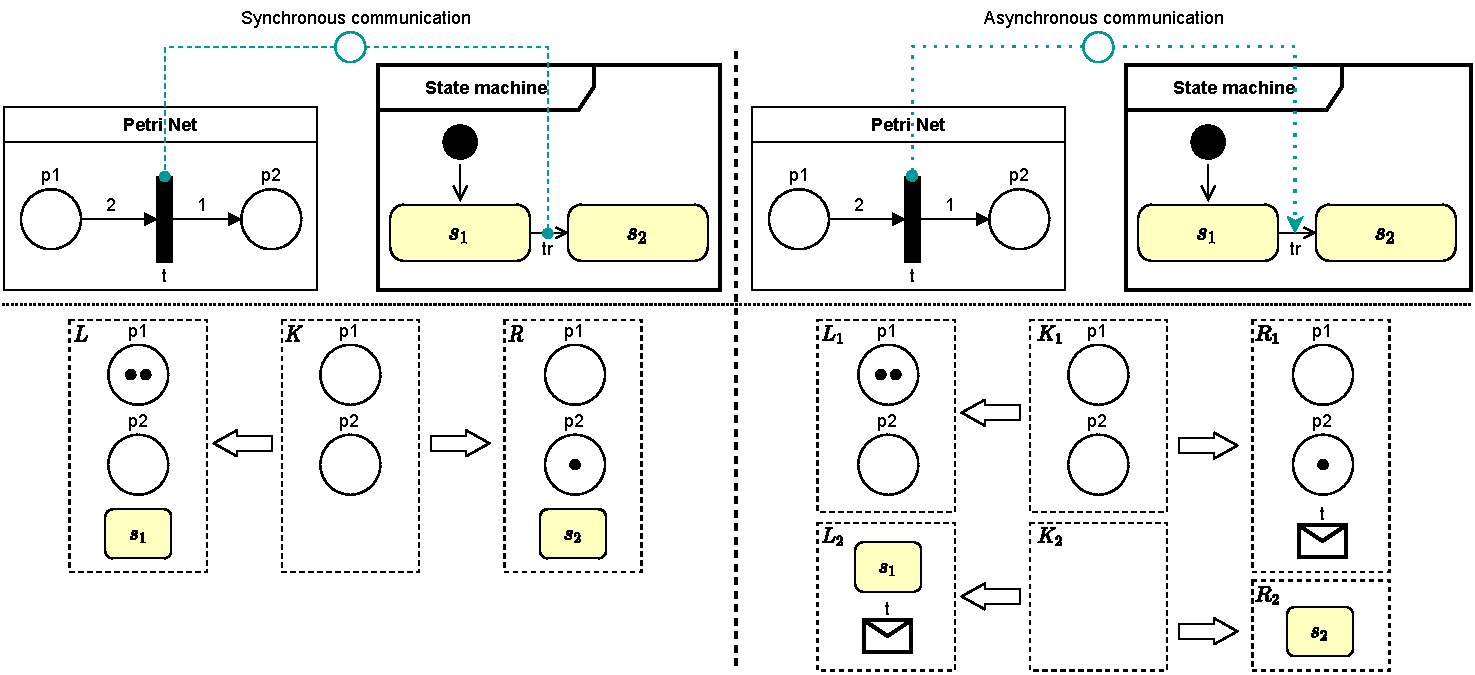
\includegraphics[width=1\textwidth]{images/synch_asynch.pdf}
    \caption{\gls{gg} rules for synchronous and asynchronous interactions}
    \label{fig:synchAsynchInteractions}
\end{figure}

Asynchronous communication will lead to rules being enriched not merged.
An asynchronous interaction has a direction and links only two model elements.
It will lead to the creation and consumption of a unique message node. 
An example can be seen on the right of \autoref{fig:synchAsynchInteractions}.
Asynchronous communication influences the global system behavior by forcing two previously unrelated rules to be executed in a certain order.

% Include the structural aspects to have multiple instances of a model without repeating it (if the same communication protocol is used between these models).

% This can be used to define hierarchical models (add some example here). State machine where a state is realised by an activity diagram or something like that.

% Overall system can be executed and properties can be checked on the state space generated by the graph grammar (link to my models paper for more information on how to do this in detail).

\section{Use case: hierarchical composition}
Highlight the approach by implementing a simple example of hierarchical composition
% Use some github repo to implement an example of the whole fiesta in groove. Maybe the hierarchical composition.

\begin{figure}[h]
    \centering
    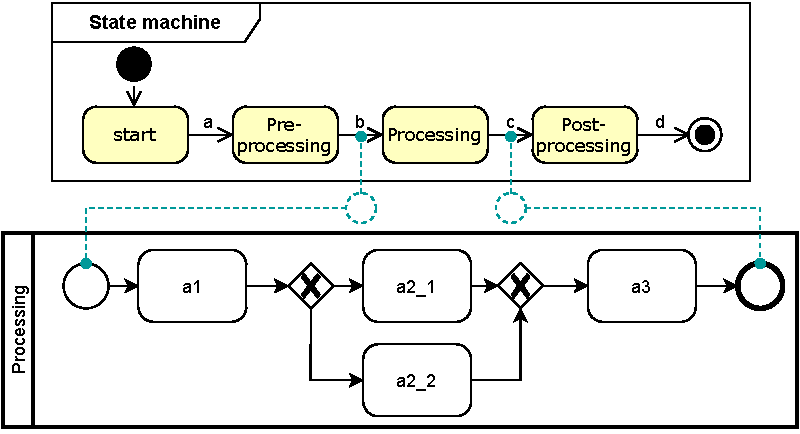
\includegraphics[width=.5\textwidth]{images/usecase.pdf}
    \caption{Hierarchical composition of a state machine and a \gls{bpmn} process model}
    \label{fig:useCase}
\end{figure}

\section{Related work}
This contribution extends our work in \cite{krauterBehavioralConsistencyHeterogeneous2021} by adding asynchronous communication and TODO.
% maybe structural aspects
% maybe new use case: hierarchical composition
% maybe new modelling language bpmn?

In \cite{kienzleUnifyingFrameworkHomogeneous2019} event structures with event scheduling are proposed to realize behavioral combination.
The authors also convert each behavioral model to their chosen formalism (event structures instead of \glspl{gg}) and combine the models in that formalism.
The combination is based on event scheduling, i.e., adding causal relations between the events of the event structures representing the behavioral models.
This will then lead to an event structure describing the behavior of the composite system similar to our approach.

% we stay closer to the original models: visualization of execution and counterexample should be easier. Since the step back to the original language is not that far.

% Parallels between event structures as their underlying formalism and my approach.
% Try to argue why my approach might be better (including dataflow in the future, data can be modelled by graphs which we operate on and can exchange easily. Visualization of the execution is easier since GG operate directly in the source language, when checking properties visualizing counterexamples if properties are not fulfilled is also easier.)

\section{Acknowledgments} \label{sect:acks}
The author would like to thank his supervisors Adrian Rutle, Harald König, and Yngve Lamo for fruitful discussions about the topic.
\label{sect:bib}
\bibliographystyle{plain}
%\bibliographystyle{alpha}
%\bibliographystyle{unsrt}
%\bibliographystyle{abbrv}
\bibliography{bib}

%------------------------------------------------------------------------------
% Index
%\printindex

%------------------------------------------------------------------------------
\end{document}

